\documentclass[10pt,journal,compsoc]{IEEEtran} % For IEEE Journal

\usepackage{graphics}
\graphicspath{ {Figures/} }
\usepackage{float}
\usepackage{balance}
\usepackage{times}
\usepackage{url}
\usepackage{subfigure}
\usepackage{color}
\usepackage[pdftex]{hyperref}
\usepackage{subfigure}
\usepackage{textcomp}
\usepackage{color}
\usepackage{capt-of}
\usepackage{mathtools}
\usepackage{amsmath}
\usepackage{algorithm,algorithmic}
\usepackage{multirow}
\usepackage{soul}

\usepackage{times}
% To make various LaTeX processors do the right thing with page size.


% End of preamble. Here it comes the document.

\begin{document}

\title{Machine Learning on Optimizing Algorithms on Tree Decomposition}

\author{Zhiyuan Shen,
Yifei Wang,
Nuo Zheng
}


\IEEEtitleabstractindextext{%
\begin{abstract}
NP problems are one of the most famous problem in the theoretical computer science aspect. The exponential time complexity makes it unsolvable if the data is large. However, many methods are found to reduce the problem scale of the origin problem, including tree-decomposition. Different tree-decomposition cost different run times. However, we can fastly generate tree-decompositions \cite{BHL1996LinearTreeDeomposition}, that means, if choose the best tree-decomposition, the run time of program can be reduce a lot. Our goal is to do the further optimization based on the tree-decompositions.
\end{abstract}

% Note that keywords are not normally used for peerreview papers.
% add keywords here
% \begin{IEEEkeywords}
% Here goes keywords.
% \end{IEEEkeywords}
}

\maketitle

\section{Introduction}~\label{sec.introduction}

This paper aims to use the machine learning to predict the run time of 3-colorability on a graph and its tree-decomposition. Thus we can generate multiple tree-decomposition, and find the fastest one then solve it.

This project chooses the 3-colorability as an example because it is a relatively easy NP-complete problem. This paper may first introducing some background information and give a fully view of how the project built.

This project conducts 3 parts, including data generating part, machine learning part and final test part. All 3 parts will be fully explained below analyses.

In conclusion, the paper will show the findings of optimization through machine learning on the tree-decompositions and try to explain the reasons behind such result.
\section{Related Works}~\label{sec.relatedworks}

From the basic algorithm, the most traditional algorithm is to enumerate the colors of all nodes. After that, graph-coloring problem is determined to be the NP-complete problem. Rather than solve the problem straightforward, academic circle tries to reduce the scale of the problem. Tree-decomposition is an effective method\cite{BasicTD1991} to reduce the scale of origin problem.

Then, the focus is shifted to the problems on the tree-decompositions. Improved tree-decomposition methods are found \cite{BHL1996LinearTreeDeomposition}\cite{BHL1991BetterAlgoTreeWidth}\cite{FasterTD2019} to form a more standard and solvable structures.

Next, machine learning was introduced into this problem \cite{MLonTD2017}. Machine learning is used to predict the run time of tree-decomposition structure and help problem-solver to dicide to solve which structure.
\section{Background Information}~\label{sec.background}

This section will introduce 3 basci concept of the project, 3-colorability, Tree-decomposition, and machine-learning.

\subsection{3-colorability}~\label{sec.subbackground1}

A coloring of a graph refers to a proper vertex coloring, namely a labeling of the graph's vertices with colors such that no two vertices sharing the same edge have the same color.

A coloring using at most k colors is called a proper $k$-coloring. Thus if $k\le 3$, we call the graph is 3-colorable.

The same, if a graph $G=(V, E)$ is 3 colorable. There should exist one example that $\forall v \in V, color(v) \in \{R, B, G\}$, and $\forall e = (u, v) \in E, color(u) != color(v)$.

\subsection{Tree Decomposition}~\label{sec.subbackground2}

A \textit{tree decomposition} of a graph $G=(V, E)$ is a tree $T$, where

\begin{enumerate}
    \item Each vertex $i$ of $T$ is labeled by a subset $B_{i} \subset V$ of vertices $G$, referred to as a "bag".
    \item Each edge of $G$ is in a subgraph induced by at least one of the $B_{i}$
    \item $\forall u \in V$, The subtree of $T$ consisting of all "bags"containing $u$ is connected.
\end{enumerate}

A rooted \textit{nice tree decomposition} $(T, B)$ of a graph $G=(V, E)$ is \textit{nice} if each node $x$ of $T$ is of one of the following types:

\begin{enumerate}
    \item leaf node: $x$ has no children and $|B_{x}| = 1$.
    \item introduce node: $x$ has a unique child $y$ and $B_{x}=B_{y}\cup\{v\}$ for some $v \in V \backslash B_{y}$.
    \item forget node: $x$ has a unique child $y$ and $B_{x}=B_{y}\backslash\{v\}$ for some $v \in B_{y}$.
    \item join node: $x$ has exactly 2 children $y, z$ and $B_{x}=B_{y}=B_{z}$
\end{enumerate}

We can convert a given tree decomposition of width $t$ and $O(n)$ nodes into a nice
tree decomposition of width $t$ and $O(tn)$ nodes in time $t^{O(1)}n$\cite{FasterTD2019}.

\subsection{Machine Learning and Predictions}
\section{Data-Set Generating}~\label{sec.DataGen}

This project generate all the data in Linux, Ubuntu 20.04 environment. The code could be found at \url{https://github.com/jerry3128/Stats102-Final-Project-Linux}.

In total, we generate 2000 graphs and 100 tree decompositions for each graph used to train our model. The cloud server location is 124.223.218.55.

\subsection{Graph Generating}~\label{sec.DataGen1}

The undirected graph is generated based on uniformly randomly select the edge from the complete graph. In this way, it is convenient to control some features like the number of edges.

\subsection{Tree Decomposition Generating}~\label{sec.DataGen2}

In this part, the implemention refers to hypertree decompositions(\url{https://github.com/mabseher/htd}), and \cite{BHL1996LinearTreeDeomposition}. Thus the tree-decomposition algorithm for this project is actually a combined algorithm.

In the process of generating tree-decomposition, we may find a maximum matching of the graph, and we can adjust the tree-decomposition after we done the algorithm, thus we can randomize the order to node to get different tree decomposition and add slight variables to the tree-decomposition to generate mutiple of them.

\subsection{Problem Solver}~\label{sec.DataGen3}

To solve the 3-colorability on a graph with its tree-decomposition, we may use ASP (Answer Set program) principles \cite{ASP2008}.

Originally, we have the full set of answers. For 3-colorability, that means we can color every node into every color. When we gradually link the edges, new restrictions, such as the color of two nodes in a link cannot be the same, will be formed. Then, we delete the answers in the set that do not satisfy the new restrictions.

In the end, the remained answers are acceptable answers to origin problem.

To implement this algorithm, we can use back-track searching through C++ to stimulate the process. More information could be found in the code.

\subsection{CSV File Generating}~\label{sec.DataGen4}

Another C++ program is written to generate csv file and deal with these features.
\section{Machine Learning}~\label{sec.ML}

In this section, we will introduce the features we select and how we implement the machine learning.

Apparently, compared to the other features, the \textit{Tree Width} has much more impact on the run time. Thus we straightly group the data by tree width, and then for each group we do the polynomial linear regression.

Here is the features we may use:

\begin{enumerate}
    \item Average Bag Size: Average of size of bags on tree decomposition.
    \item Decomposition Overhead Ratio: Sum of bag size divided by size of graph.
    \item Average Depth: Average depth of tree.
    \item Node percentage: Introduce/Forget/Join/Leaf's Percentage of tree (sum of them is 100\%).
    \item Sum of Join node distance: Find all pairs of Join nodes and plus their distances.
    \item Branching Factor: Average number of childs (exclude leaf nodes).
    \item Bag Adjacency Factor: For all pair of nodes in a bag, that the adjacencent pairs divided by the total pairs.
    \item Bag Connectedness Factor: For all pair of nodes in a bag, the reachable pairs divided by the total pairs.
    \item Bag Neighborhood Coverage Factor: For all bags $B_{x}$, average of nodes that belong to a bag $B_{x}$ or are adjacencent to a node belongs to $B_{x}$
\end{enumerate}

After training, we use cross validation to validate each model and select the polynomial linear regression.

We select the best models to participate in the final test.

Model: For each tree width, we use Linear-Regression to predict the runtime.

\begin{figure}[h!]
    \centering
    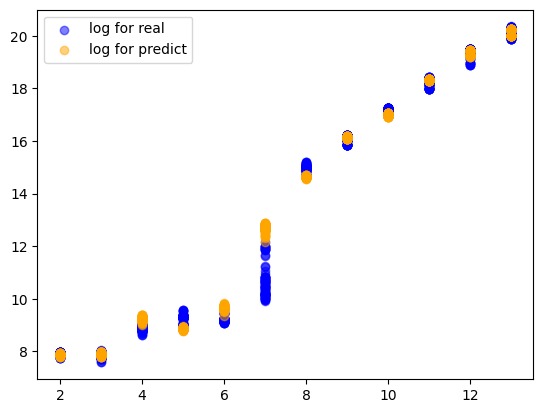
\includegraphics[width=0.36\textwidth]{model_polyLR.png}
    \caption{separate tree-width, straight polynomial linear regression for run time}
    \label{separate tree-width, straight polynomial linear regression for run time}
    \end{figure}

Also we compare this model with the other models by the square of the difference between the predictions and real value, and we call this.

The models for the ln of run time all has sum of square of difference over $10^{6}$, while straightly linear regression the run time only over $10^{5}$.

Then, we see that, if we combine all data, the model shows obvious inaccurate in the area that tree width is little.

\begin{figure}[h!]
    \centering
    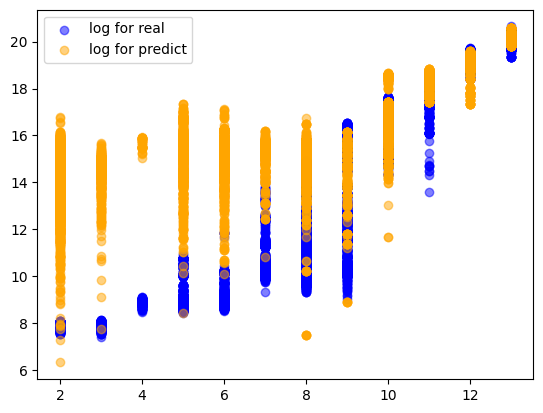
\includegraphics[width=0.36\textwidth]{no_separate_treewidth.png}
    \caption{combine tree-width, straight polynomial linear regression for run time}
    \label{combine tree-width, straight polynomial linear regression for run time}
    \end{figure}

Thus we may choose the separate tree width model as the predictor.
\section{Conclusion}~\label{sec.Conclusion}

In this section, we compare efficiency of the
\begin{enumerate}
    \item \textit{predictor 1: machine learning predictor}.
    \item \textit{predictor 2: theory time complexity predictor}.
    \item \textit{predictor 3: average running time}.
\end{enumerate}
to solve new generated graphs.

We will analysis the result and provide the further project focus.

\begin{figure}[h!]
    \centering
    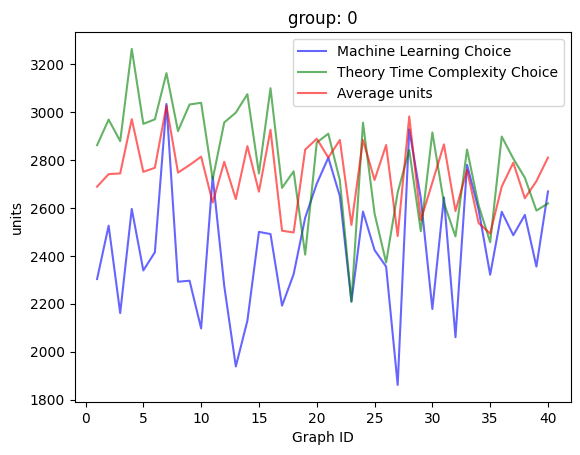
\includegraphics[width=0.36\textwidth]{result-1.png}
    \caption{combine tree-width, straight polynomial linear regression for run time}
    \label{combine tree-width, straight polynomial linear regression for run time}
    \end{figure}

The \textit{predictor 1} shows a very high performance averagely. That only cost 87.4\% run time of \textit{predictor 2} and 91.0\% run time of \textit{predictor 3}.

However, here is 2\% for this predictor that get huge differences, that the predicted run time is 2 times larger than real run time. Also, we found that the optimization is not so well when the tree width is large, and the efficiency smaller than related works.

We thought that, still the predictor has not sufficient data to do learning, especially in the large tree width area. Also, we found that our tree decomposition algorithm is a kind of combined algorithm, so that it is not uniformly random and will have a higher probability to already optimized tree decomposition.

Thus we may improve our project by constantly adding data and improve the basic algorithm parts.

\bibliographystyle{abbrv}
\bibliography{References.bib}

\end{document}
